% ===========================================================================
% Part V - Neural Networks: Multilayer Perceptron (Experiment 13)
% ===========================================================================

\part{Neural Networks: Multilayer Perceptron}

% ---------------------------------------------------------------------------
\chapter{Experiment 13: Multilayer Perceptron (MLP)}\label{exp:13}

\quickfacts
  {Dataset}{Digits (scikit-learn): 1,797 samples, 8$\times$8 images (64 features), 10 classes; 70/15/15 split}
  {Key parameters}{scikit-learn (128, 64) ReLU + Adam + early stopping; PyTorch 64--128--64--10 with BatchNorm and Dropout}
  {Headline result}{scikit-learn 0.9630; PyTorch 0.9815 test accuracy (GPU)}

\section{Objective}
Implement feed-forward neural networks for handwritten-digit classification and study
hidden-layer size and regularization.

\section{Suggested Dataset}
Digits (scikit-learn): 1,797 samples, 8$\times$8 grayscale images (64 features), 10 classes;
stratified 70/15/15 train/validation/test split, standardized on the training data only.

\section{Required Libraries}
scikit-learn, PyTorch, numpy, pandas, matplotlib.

\section{Brief Theory}
An MLP stacks affine transformations with non-linear activations,
\[
a^{(l)} = \sigma\bigl(W^{(l)} a^{(l-1)} + b^{(l)}\bigr), \qquad
\hat{y} = \mathrm{softmax}\bigl(W^{(L+1)} a^{(L)} + b^{(L+1)}\bigr),
\]
and is trained by backpropagation to minimize the categorical cross-entropy
\[
\mathcal{L} = -\sum_{i=1}^{N}\sum_{k=1}^{K} y_{ik}\ln \hat{y}_{ik}
              + \frac{\alpha}{2}\sum_{l}\lVert W^{(l)}\rVert_F^2 .
\]
\textbf{Batch normalization} stabilizes layer inputs and speeds training, \textbf{dropout}
randomly zeroes neurons to regularize, and \textbf{early stopping} / learning-rate scheduling
stop training when validation performance stalls.

\section{Procedure}
\begin{enumerate}
  \item Load the digits, split 70/15/15 and standardize (fit on training data only).
  \item Train a scikit-learn \texttt{MLPClassifier} with hidden layers (128, 64), ReLU, Adam,
        $L_2$ regularization and early stopping.
  \item Build a custom PyTorch MLP: 64--128--64--10 with BatchNorm and Dropout, cross-entropy
        loss, Adam with weight decay, 50 epochs and a plateau scheduler.
  \item Train with the validation loop and plot the loss curve.
  \item Evaluate the test set and report the per-class classification report.
\end{enumerate}

\section{Reference Implementation}
\begin{lstlisting}[style=mlcode,caption={The two MLP architectures}]
mlp_sklearn = MLPClassifier(hidden_layer_sizes=(128, 64), activation='relu', solver='adam',
                            alpha=0.001, batch_size=64, learning_rate_init=0.005,
                            max_iter=150, early_stopping=True, validation_fraction=0.15)

self.net = nn.Sequential(
    nn.Linear(64, 128), nn.BatchNorm1d(128), nn.ReLU(), nn.Dropout(0.25),
    nn.Linear(128, 64), nn.BatchNorm1d(64),  nn.ReLU(), nn.Dropout(0.20),
    nn.Linear(64, 10))
\end{lstlisting}

\section{Evaluation / Expected Output}
\begin{table}[htbp]
  \centering
  \caption{MLP implementations on the digits test set (270 images).}
  \begin{tabular}{@{}lrl@{}}
    \toprule
    \textbf{Model} & \textbf{Test accuracy} & \textbf{Notes} \\
    \midrule
    Scikit-learn MLP (128--64) & 0.9630 & early stopping after 15 iterations \\
    PyTorch deep MLP & \best{0.9815} & GPU (CUDA), 50 epochs, validation accuracy 0.9889 \\
    \bottomrule
  \end{tabular}
\end{table}

\begin{figure}[htbp]
  \centering
  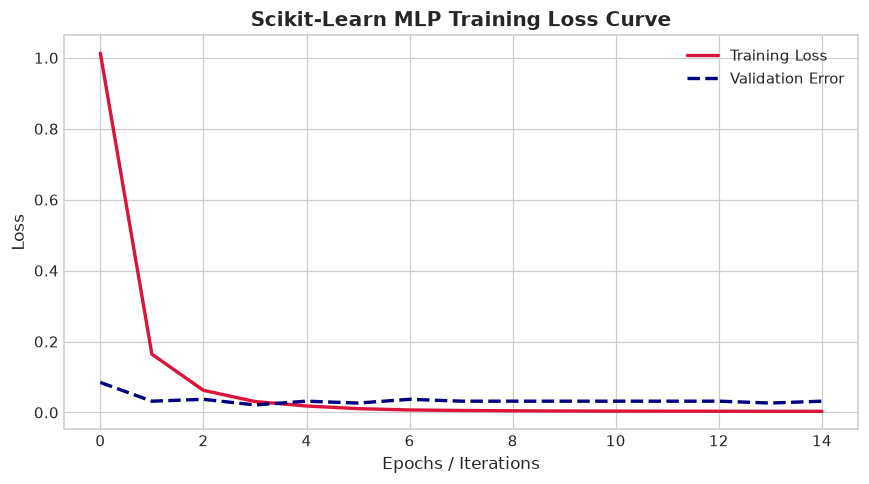
\includegraphics[width=0.75\textwidth]{figures/exp13_sklearn_loss.png}
  \caption{Training loss curve of the scikit-learn MLP; early stopping halted training after
  15 iterations.}
  \label{fig:exp13-loss}
\end{figure}

Training loss fell from 1.20 to about 0.02 while the validation loss tracked it closely, so
there is no severe overfitting. Per-class precision and recall are near 1.00 for almost all
digits; the residual errors are visually similar digits. The custom PyTorch model beats the
scikit-learn baseline by about two points thanks to BatchNorm, Dropout and scheduled training
over more epochs.

\section{Viva / Discussion Questions}
\begin{description}
  \item[Why is scaling important for MLP?] Gradient descent converges poorly when input
  features have very different scales; standardization equalizes their influence and stabilizes
  the loss surface.
  \item[What is backpropagation?] Reverse-mode application of the chain rule that computes the
  gradient of the loss with respect to every weight, layer by layer.
  \item[What causes vanishing/exploding gradients?] Repeated multiplication of small (or
  large) Jacobians through many layers; ReLU, BatchNorm, careful initialization and residual
  connections mitigate it.
  \item[Why is the PyTorch model better here?] BatchNorm and Dropout plus a longer, scheduled
  training; the scikit-learn model stops early at iteration 15.
\end{description}

\section{Complete Code Listing}
% ===========================================================================
% exp13_mlp.tex - complete code listings for Experiment 13
% Source: notebooks/05_multilayer_perceptron.ipynb (executed)
% Repository: https://github.com/Atik203/ML-Algorithms
% ===========================================================================

\begin{codebox}[title={Core numerical and plotting libraries}]
# ---- Core numerical and plotting libraries ----
import numpy as np
import pandas as pd
import matplotlib.pyplot as plt
import seaborn as sns

# ---- Dataset + preprocessing/metrics ----
from sklearn.datasets import load_digits
from sklearn.model_selection import train_test_split
from sklearn.preprocessing import StandardScaler
# ---- Scikit-Learn MLP implementation ----
from sklearn.neural_network import MLPClassifier
from sklearn.metrics import accuracy_score, classification_report, confusion_matrix

# ---- PyTorch for the custom deep MLP ----
import torch
import torch.nn as nn
import torch.optim as optim
from torch.utils.data import DataLoader, TensorDataset

# Styling setup (consistent look across all notebooks)
plt.style.use('seaborn-v0_8-whitegrid' if 'seaborn-v0_8-whitegrid' in plt.style.available else 'default')
plt.rcParams['font.sans-serif'] = 'DejaVu Sans'
plt.rcParams['figure.figsize'] = (10, 6)
plt.rcParams['figure.dpi'] = 110

# Fix seeds for reproducible training
torch.manual_seed(42)
torch.cuda.manual_seed_all(42)  # reproducible GPU training
np.random.seed(42)
print(f"PyTorch version: {torch.__version__}")
device = torch.device('cuda' if torch.cuda.is_available() else 'cpu')  # use GPU if available
print(f"Computation Device: {device}")

# ---- Load the handwritten digits dataset (8x8 grayscale images) ----
digits = load_digits()
X_raw = digits.data      # flattened images: 1797 samples x 64 pixel features
y = digits.target        # digit class 0..9

print(f"Dataset Shape: {X_raw.shape}, Target Classes: {np.unique(y)}")
# ---- Train / Validation / Test split (70% / 15% / 15%) ----
# First cut off the test set...
X_train_val, X_test, y_train_val, y_test = train_test_split(
    X_raw, y, test_size=0.15, random_state=42, stratify=y
)
# ...then split the remainder into train and validation
X_train, X_val, y_train, y_val = train_test_split(
    X_train_val, y_train_val, test_size=0.1765, random_state=42, stratify=y_train_val
)

# ---- Feature scaling: fit on training data only (avoid validation/test leakage) ----
scaler = StandardScaler()
X_train_scaled = scaler.fit_transform(X_train)
X_val_scaled = scaler.transform(X_val)
X_test_scaled = scaler.transform(X_test)

print(f"Training samples:   {X_train_scaled.shape[0]}")
print(f"Validation samples: {X_val_scaled.shape[0]}")
print(f"Test samples:       {X_test_scaled.shape[0]}")
\end{codebox}

\begin{codebox}[title={Scikit-Learn MLPClassifier: 64 -> 128 -> 64 -> 10}]
# ---- Scikit-Learn MLPClassifier: 64 -> 128 -> 64 -> 10 ----
mlp_sklearn = MLPClassifier(
    hidden_layer_sizes=(128, 64),   # two hidden layers
    activation='relu',
    solver='adam',                  # adaptive gradient optimizer
    alpha=0.001,                    # L2 regularization strength
    batch_size=64,
    learning_rate_init=0.005,
    max_iter=150,
    early_stopping=True,            # stop when validation score stops improving
    validation_fraction=0.15,       # internal validation split for early stopping
    random_state=42
)

# Train (forward pass + backpropagation happen inside .fit)
mlp_sklearn.fit(X_train_scaled, y_train)

# Evaluate on the untouched test set
y_pred_sk = mlp_sklearn.predict(X_test_scaled)
acc_sk = accuracy_score(y_test, y_pred_sk)

print(f"Scikit-Learn MLP Test Accuracy: {acc_sk:.4f}")
print(f"Converged after {mlp_sklearn.n_iter_} iterations")

# ---- Plot the training loss curve recorded by scikit-learn ----
plt.figure(figsize=(8, 4.5))
plt.plot(mlp_sklearn.loss_curve_, color='crimson', lw=2.2, label='Training Loss')
if hasattr(mlp_sklearn, 'validation_scores_'):
    # validation_scores_ stores accuracy; convert to error for a comparable scale
    plt.plot([1 - s for s in mlp_sklearn.validation_scores_], color='navy', lw=2.2, linestyle='--', label='Validation Error')
plt.title("Scikit-Learn MLP Training Loss Curve", fontsize=13, fontweight='bold')
plt.xlabel("Epochs / Iterations", fontsize=11)
plt.ylabel("Loss", fontsize=11)
plt.legend()
plt.tight_layout()
plt.show()
\end{codebox}

\begin{codebox}[title={Convert scaled NumPy arrays into PyTorch tensors + DataLoaders}]
# ---- Convert scaled NumPy arrays into PyTorch tensors + DataLoaders ----
train_dataset = TensorDataset(torch.tensor(X_train_scaled, dtype=torch.float32), torch.tensor(y_train, dtype=torch.long))
val_dataset   = TensorDataset(torch.tensor(X_val_scaled, dtype=torch.float32),   torch.tensor(y_val, dtype=torch.long))
test_dataset  = TensorDataset(torch.tensor(X_test_scaled, dtype=torch.float32),  torch.tensor(y_test, dtype=torch.long))

# DataLoaders handle mini-batching and shuffling during training
train_loader = DataLoader(train_dataset, batch_size=32, shuffle=True)
val_loader   = DataLoader(val_dataset, batch_size=64, shuffle=False)
test_loader  = DataLoader(test_dataset, batch_size=64, shuffle=False)

class DeepMLP(nn.Module):
    """Fully-connected classifier: 64 -> 128 -> 64 -> 10 with BatchNorm + Dropout."""
    def __init__(self, in_features=64, num_classes=10):
        super(DeepMLP, self).__init__()
        self.net = nn.Sequential(
            # Hidden block 1
            nn.Linear(in_features, 128),
            nn.BatchNorm1d(128),    # stabilizes activations, speeds up training
            nn.ReLU(),              # non-linear activation
            nn.Dropout(0.25),       # regularization: randomly drop 25% of neurons

            # Hidden block 2
            nn.Linear(128, 64),
            nn.BatchNorm1d(64),
            nn.ReLU(),
            nn.Dropout(0.20),

            # Output layer: 10 raw logits (one per digit class)
            nn.Linear(64, num_classes)
        )

    def forward(self, x):
        return self.net(x)

model = DeepMLP().to(device)   # move all parameters to CPU/GPU
print(model)
\end{codebox}

\begin{codebox}[title={Training configuration}]
# ---- Training configuration ----
criterion = nn.CrossEntropyLoss()                                            # softmax + NLL loss
optimizer = optim.Adam(model.parameters(), lr=0.003, weight_decay=1e-4)      # weight decay = L2
scheduler = optim.lr_scheduler.ReduceLROnPlateau(optimizer, mode='min', factor=0.5, patience=5)

epochs = 50
history = {'train_loss': [], 'val_loss': [], 'train_acc': [], 'val_acc': []}

for epoch in range(epochs):
    # ---------- Training phase ----------
    model.train()                          # enable Dropout/BatchNorm training behavior
    running_loss, correct, total = 0.0, 0, 0
    for inputs, labels in train_loader:
        inputs, labels = inputs.to(device), labels.to(device)

        optimizer.zero_grad()              # reset gradients from the previous step
        outputs = model(inputs)            # forward pass
        loss = criterion(outputs, labels)  # compute cross-entropy
        loss.backward()                    # backpropagation (compute gradients)
        optimizer.step()                   # update weights

        # Accumulate metrics (loss is averaged over the batch, so multiply by batch size)
        running_loss += loss.item() * inputs.size(0)
        _, preds = torch.max(outputs, 1)   # predicted class = highest logit
        correct += (preds == labels).sum().item()
        total += labels.size(0)

    epoch_train_loss = running_loss / total
    epoch_train_acc = correct / total

    # ---------- Validation phase ----------
    model.eval()                           # disable Dropout, use running BatchNorm stats
    val_loss, val_correct, val_total = 0.0, 0, 0
    with torch.no_grad():                  # no gradients needed for evaluation
        for inputs, labels in val_loader:
            inputs, labels = inputs.to(device), labels.to(device)
            outputs = model(inputs)
            loss = criterion(outputs, labels)

            val_loss += loss.item() * inputs.size(0)
            _, preds = torch.max(outputs, 1)
            val_correct += (preds == labels).sum().item()
            val_total += labels.size(0)

    epoch_val_loss = val_loss / val_total
    epoch_val_acc = val_correct / val_total
    scheduler.step(epoch_val_loss)         # reduce LR if validation loss plateaus

    # Record metrics for plotting
    history['train_loss'].append(epoch_train_loss)
    history['val_loss'].append(epoch_val_loss)
    history['train_acc'].append(epoch_train_acc)
    history['val_acc'].append(epoch_val_acc)

    # Print a progress line every 10 epochs (and the first one)
    if (epoch + 1) % 10 == 0 or epoch == 0:
        print(f"Epoch [{epoch+1:02d}/{epochs}] "
              f"Train Loss: {epoch_train_loss:.4f} | Train Acc: {epoch_train_acc:.4f} || "
              f"Val Loss: {epoch_val_loss:.4f} | Val Acc: {epoch_val_acc:.4f}")
\end{codebox}

\begin{codebox}[title={Final evaluation on the held-out test set}]
# ---- Final evaluation on the held-out test set ----
model.eval()
test_preds = []
test_targets = []

with torch.no_grad():
    for inputs, labels in test_loader:
        inputs = inputs.to(device)
        outputs = model(inputs)
        _, preds = torch.max(outputs, 1)          # predicted digit
        test_preds.extend(preds.cpu().numpy())    # move back to CPU for metrics
        test_targets.extend(labels.numpy())

acc_pytorch = accuracy_score(test_targets, test_preds)
print(f"PyTorch Deep MLP Test Accuracy: {acc_pytorch:.4f}\n")
print("Detailed Classification Report:")
# Per-class precision/recall/F1 for all 10 digits
print(classification_report(test_targets, test_preds, digits=4))
\end{codebox}

